\begin{quoting}
Baking refers to the part of the process where you are loading
your dough into the oven. This is typically done after your
dough has gone through the bulk fermentation and proofing stage.
\end{quoting}

\begin{flowchart}[!htb]
\begin{center}
  \begin{tikzpicture}[node distance = 3cm, auto]
  \node [block] (heat_oven) {\footnotesize Heat oven to 230°C (446°F) for 30 minutes};
  \node [block, right of=heat_oven, node distance=3cm] (score_dough) {\footnotesize Score your dough};
  \node [decision, right of=score_dough, node distance=4cm] (decide_steam) {\footnotesize Choose your steaming method};
  \node [block, below of=heat_oven, node distance=4cm] (inverted_tray_method) {\footnotesize Inverted tray method};
  \node [block, right of=inverted_tray_method, node distance=3cm] (dutch_oven) {\footnotesize Dutch oven};
  \node [block, right of=dutch_oven, node distance=3cm] (steam_injection) {\footnotesize Steam injection oven};
  \node [block, below of=inverted_tray_method, node distance=3cm] (bake_30) {\footnotesize Bake dough for 30 minutes with steam};
  \node [block, right of=bake_30, node distance=3cm] (remove_steam) {\footnotesize Remove source of steam};
  \node [block, right of=remove_steam, node distance=3cm] (build_crust) {\footnotesize Build the crust};
  \node [block, right of=build_crust, node distance=3cm] (finish_baking) {\footnotesize Stop baking 10--30 minutes later depending on crust preference};
  \path [line] (heat_oven) -- (score_dough);
  \path [line] (score_dough) -- (decide_steam);
  \path [line] (decide_steam) -- (inverted_tray_method);
  \path [line] (decide_steam) -- (dutch_oven);
  \path [line] (decide_steam) -- (steam_injection);
  \path [line] (steam_injection) -- (bake_30);
  \path [line] (inverted_tray_method) -- (bake_30);
  \path [line] (dutch_oven) -- (bake_30);
  \path [line] (bake_30) -- (remove_steam);
  \path [line] (remove_steam) -- (build_crust);
  \path [line] (build_crust) -- (finish_baking);
\end{tikzpicture}

  \caption[Different steaming methods]{A schematic visualization of the baking
      process using different sources of steam in a home oven.}%
  \label{fig:baking-process}
\end{center}
\end{flowchart}

Some other breads like flatbreads
could also be baked on the stove. This chapter focuses on the
home oven.

As the dough heats up, the water and acids
in your dough start to evaporate. When baking
a gluten based dough, the bubbles in your dough start to expand.
Your dough starts to vertically rise. This is called oven spring.
Your bread starts to build a crust of gel-like consistency. The crust is still
extensible and can be stretched.

\begin{table}[htp!]
    \begin{center}
        \begin{tabular}{@{}rlp{0.5\textwidth}@{}}
\toprule
\thead{°C / °F} & \thead{Stage}           & \thead{Description} \\ \midrule
60 / 140        & Sterilization           & The temperature is too hot for your microorganisms and they die.\\ 
75 / 167        & Gel building            & A gel builds on the surface persisting your dough's structure.
                                            It is still extensible and can spring in the oven.\\ 
100 / 212       & Water evaporation       & Water begins to evaporate and inflates your dough's alveoli.\\ 
118 / 244       & Acetic acid evaporation & The vinegary tasting acid starts to evaporate, sourness decreases.\\ 
122 / 252       & Lactic acid evaporation & The dairy tasting lactic acid begins to evaporate, sourness further decreases.\\ 
140 / 284       & Maillard reaction       & The Maillard reaction starts to deform starches and proteins. 
                                            The dough starts browning.\\ 
170 / 338       & Caramelization          & Remaining sugars begin to caramelize giving your bread a distinct flavor.\\ \bottomrule
\end{tabular}

        \caption[Stages of dough during backing]{The different stages that
            your dough undergoes during the baking process.}
    \end{center}
\end{table}

At around  \qty{60}{\degreeCelsius} (\qty{140}{\degF}) the microbes in your dough start to die.
There are rumors that until this happens the microbes produce
a lot of \ch{CO2}, resulting in the dough's expansion. However, this temperature
is reached quickly. Furthermore, stress makes the microbes
enter sporulation mode in order to focus on spreading genetics.
More research should be done here to validate or invalidate this
claim.

At  \qty{75}{\degreeCelsius} (\qty{167}{\degF}) the surface of your dough turns into a gel. It
holds together nicely and is still extensible. This gel is essential
for oven spring as it retains the gas of your dough very well.

At around  \qty{100}{\degreeCelsius} (\qty{212}{\degF}) the water starts to evaporate out of your
dough. If this weren't the case, your dough would taste soggy and
doughy. The higher hydration your dough has, the more water your bread
still contains after the bake. The crumb is going to taste a bit
more moist. The consistency will be different.

Another often undervalued step is the evaporation of acids. At
\qty{118}{\degreeCelsius} (\qty{244}{\degF}) the acetic acid in your dough starts to evaporate.
Shortly after at  \qty{122}{\degreeCelsius} (\qty{252}{\degF}) the lactic acid begins evaporating.
This is crucial to understand and opens a door to many interesting
ways to influence your final bread's taste. As more and more water
begins to evaporate the acids in your dough become more concentrated.
There is less water but in relation you have more acids. A shorter
bake will therefore lead to a more tangy dough. The longer you bake the bread,
the more of the water evaporates, but also ultimately the acids will follow.
They will be more concentrated. In absolute units, though, they
will become less and less. The longer you bake, the less sour
your bread is going to be. By baking you can
influence which sourness level you would like to achieve.

\begin{figure}[!htb]
  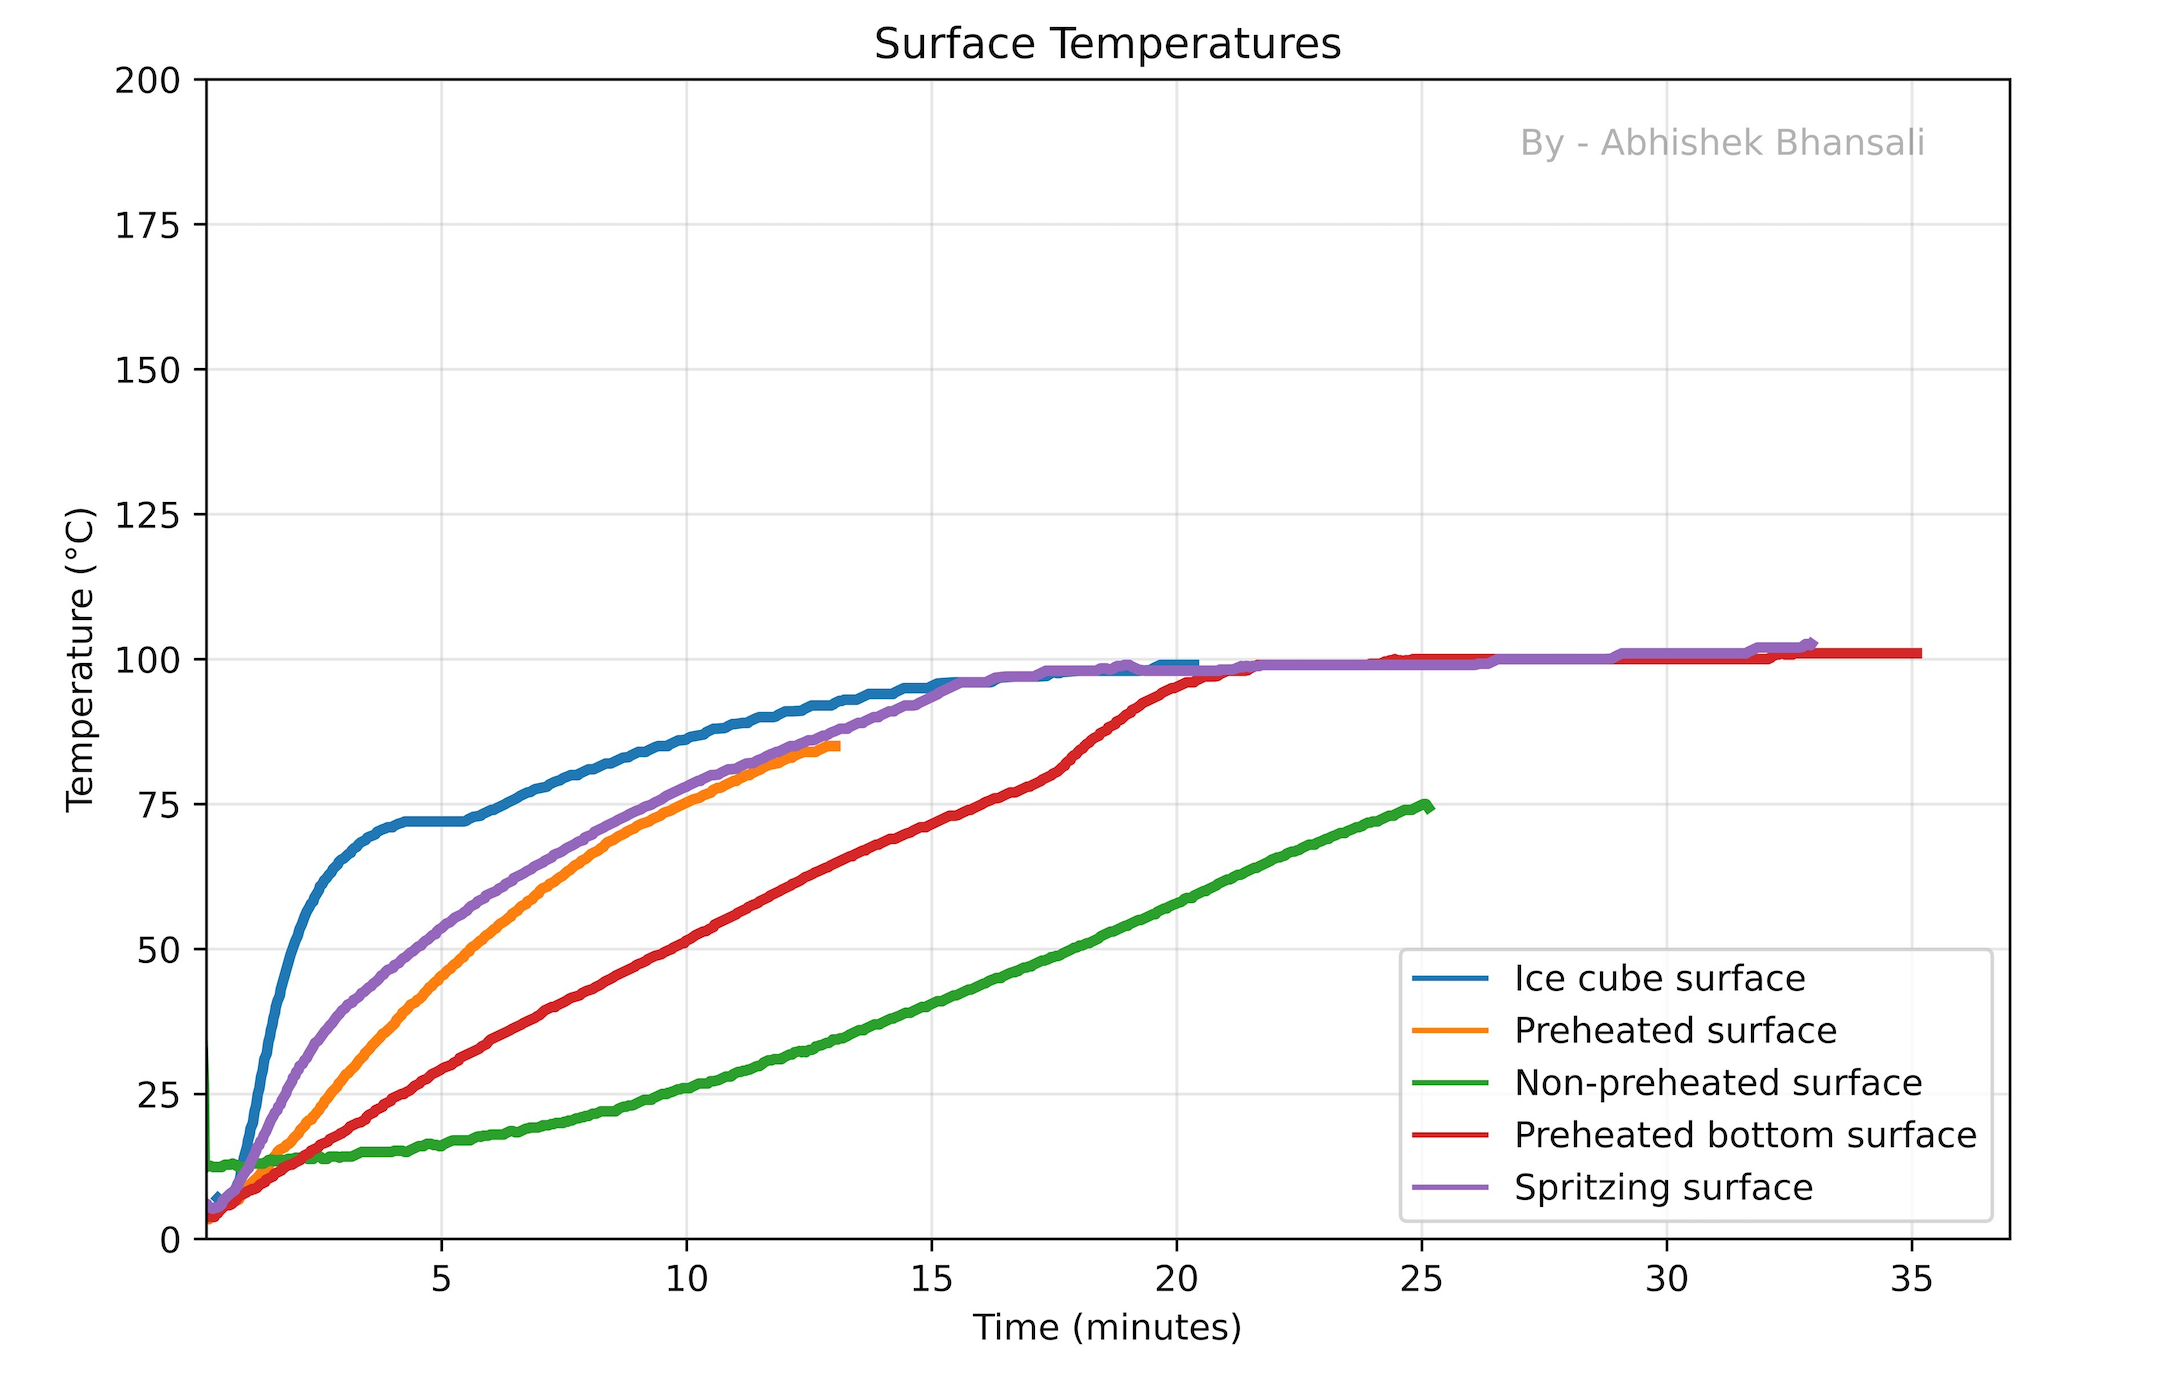
\includegraphics[width=\textwidth]{baking-experiment-temperatures.png}
  \caption[Surface temperature for different steaming methods]{This
      chart shows how surface temperatures change using different steaming
      methods. In this case I~used a Dutch oven and an apple as dough
      replacement. All the apples were coming from the fridge. The temperature
      was measured using a barbecue thermometer.  The more steam, the faster
      the surface temperature increases.}
\end{figure}

It would be a very interesting experiment to bake a bread at different exact
temperatures. How would a bread taste with only evaporated water but
full acidity? What if you were to just completely get rid of the acetic
acid? How would the taste change?

As the temperature increases
the crust thickens. The Maillard reaction kicks in, further deforming
proteins and starches. The outside of your dough starts to become
browner and crisper. This process begins at around  \qty{140}{\degreeCelsius} (\qty{284}{\degF})

Once the temperature increases even more to around  \qty{170}{\degreeCelsius} (\qty{338}{\degF}),
the caramelization process begins. The remaining sugars the microbes
did not convert yet start to brown and darken. You can keep baking
for as long as you like to achieve the crust color that you
like\footnote{This really depends a lot on your personal preference.
Some people prefer a darker crust, others prefer a more pale crust.
It's better to build less crust than too much. You can always just
heat your bread in the oven one more time to continue building a
darker crust.}.

The best method to know that your dough is done is to take
the temperature of your dough. You can use a barbecue thermometer
to measure it. Once the core temperature is at around  \qty{92}{\degreeCelsius} (\qty{197}{\degF}),
you can stop the baking process. This is typically not done though
as the crust hasn't been built yet\footnote{The thermometer is
especially important when using a large loaf pan. It is sometimes
very hard to judge from the outside if the dough is done. I~failed
many times and ended up having a semi baked dough.}.

Once your dough has finished baking, it is ready to eat. Your
dough has turned into a bread. At this
point, your bread is sterile as the temperature was too hot for
for the microorganisms to survive\footnote{I~wonder though
if a starter culture could be grown again from a slice of bread.
Under heat stress the microorganisms begin sporulating. Maybe
some of the spores survive the baking process and could be reactivated
later? If this worked, you could use any store bought sourdough
bread as a source for a new starter.}.

\section{The role of steam}

\begin{figure}[!htb]
  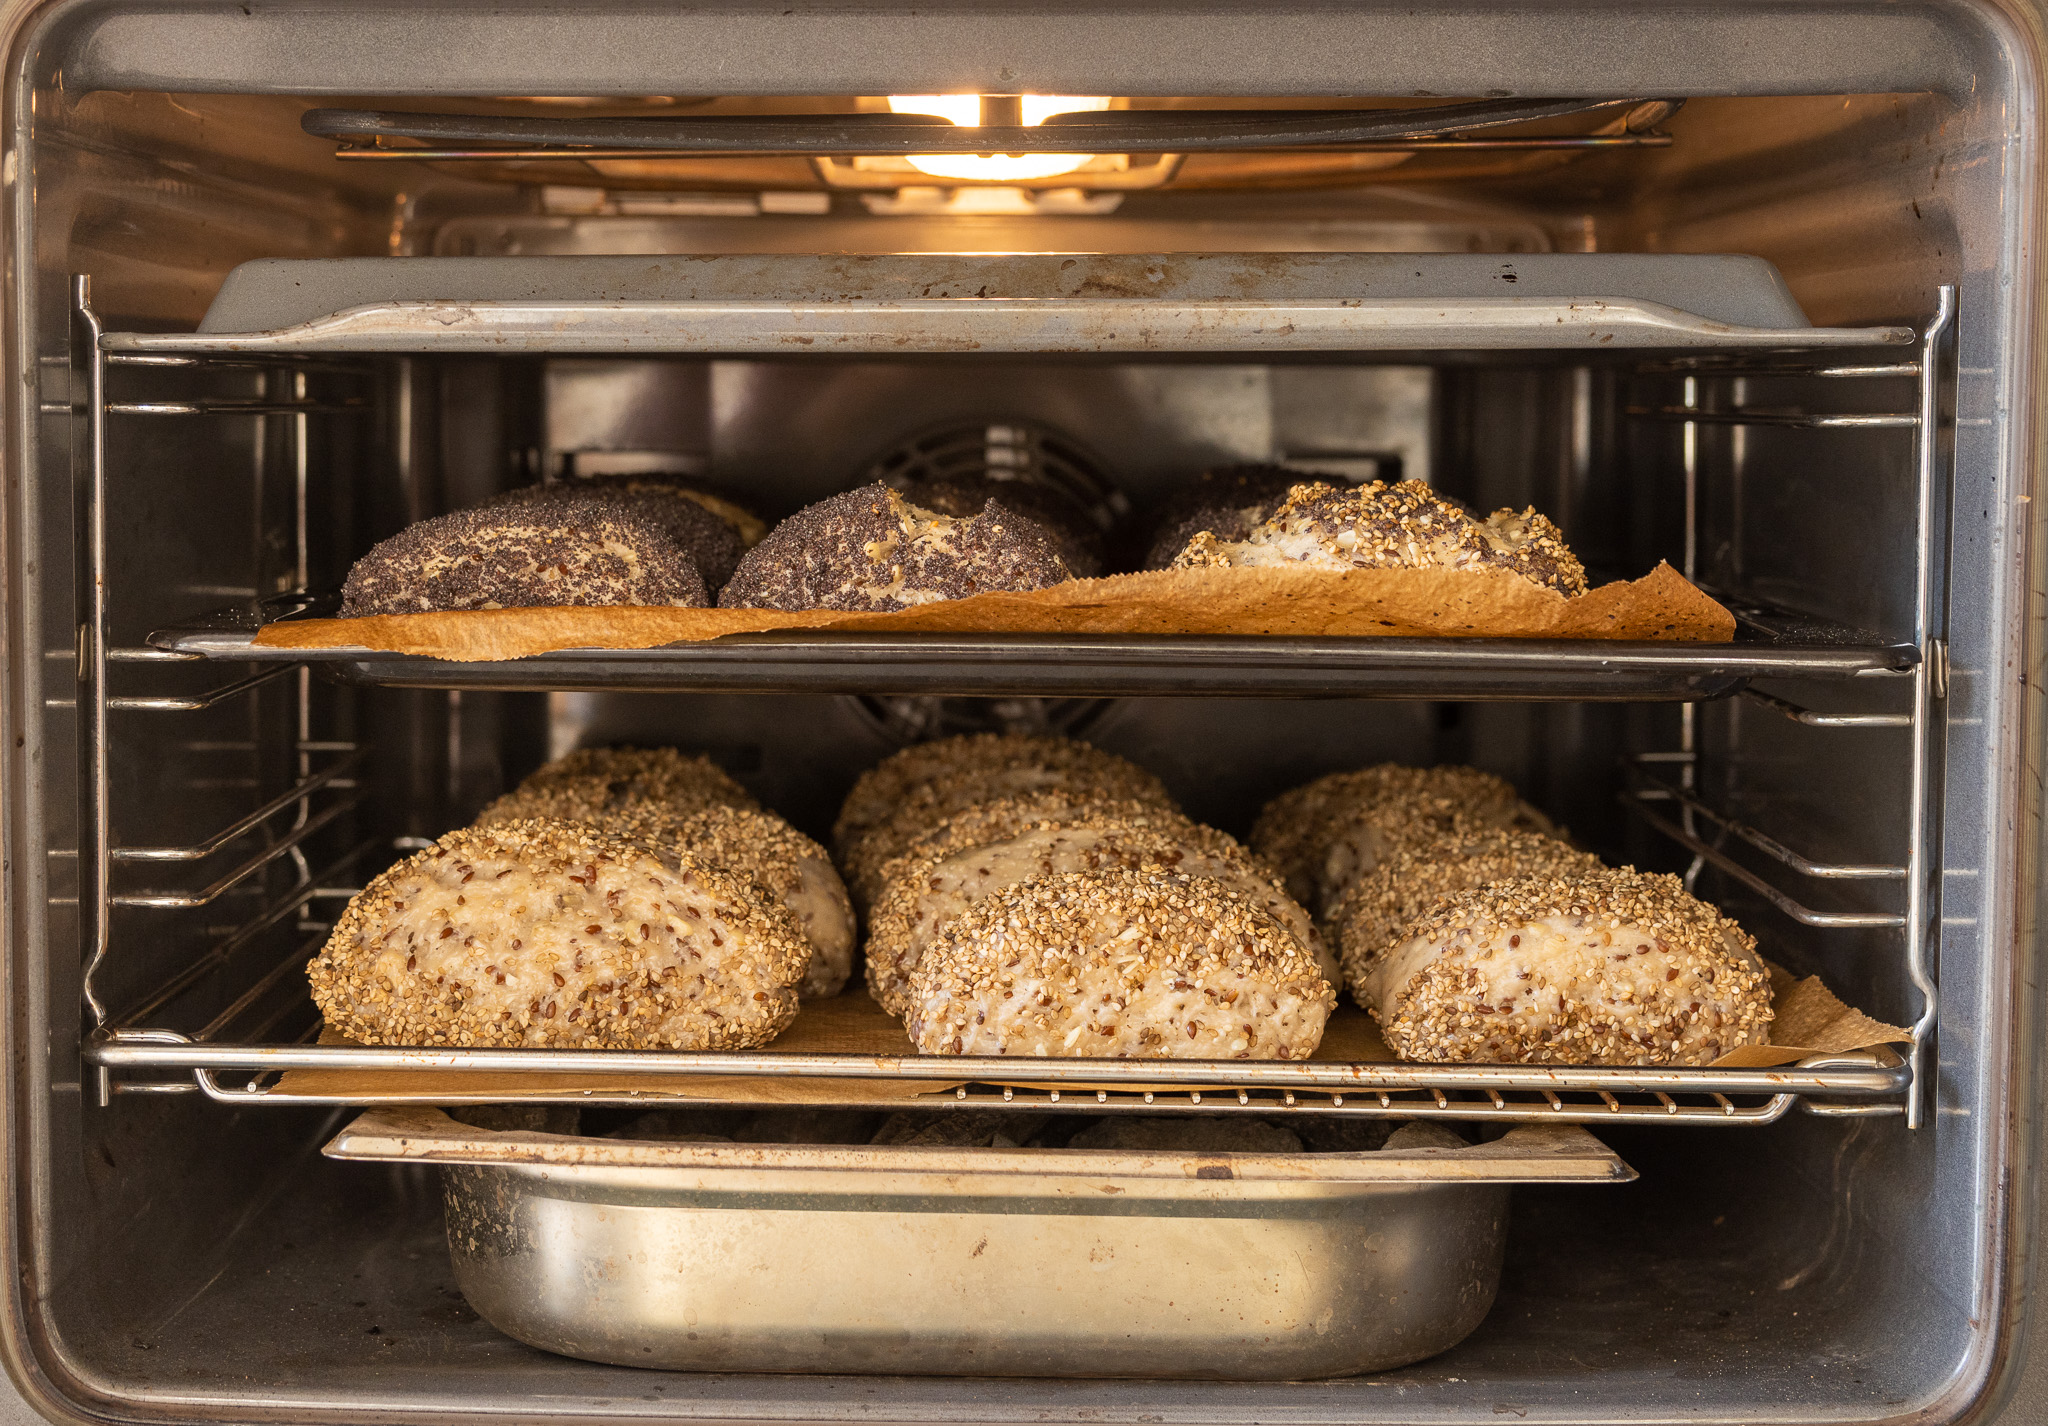
\includegraphics[width=\textwidth]{oven-example}
  \caption[Home oven baking example to maximize steam]{My default home oven setup. The tray of rocks
  and tray on top of the rolls greatly improve the steaming capabilities. This way the bread can
  rise more during the initial stage of the baking process.}
\end{figure}

Steam is essential when baking as it helps to counter premature
crust building. During the first stage of the bake, the dough
increases in size. The water in your dough evaporates and pushes
the whole dough upwards.

\begin{figure}[!htb]
  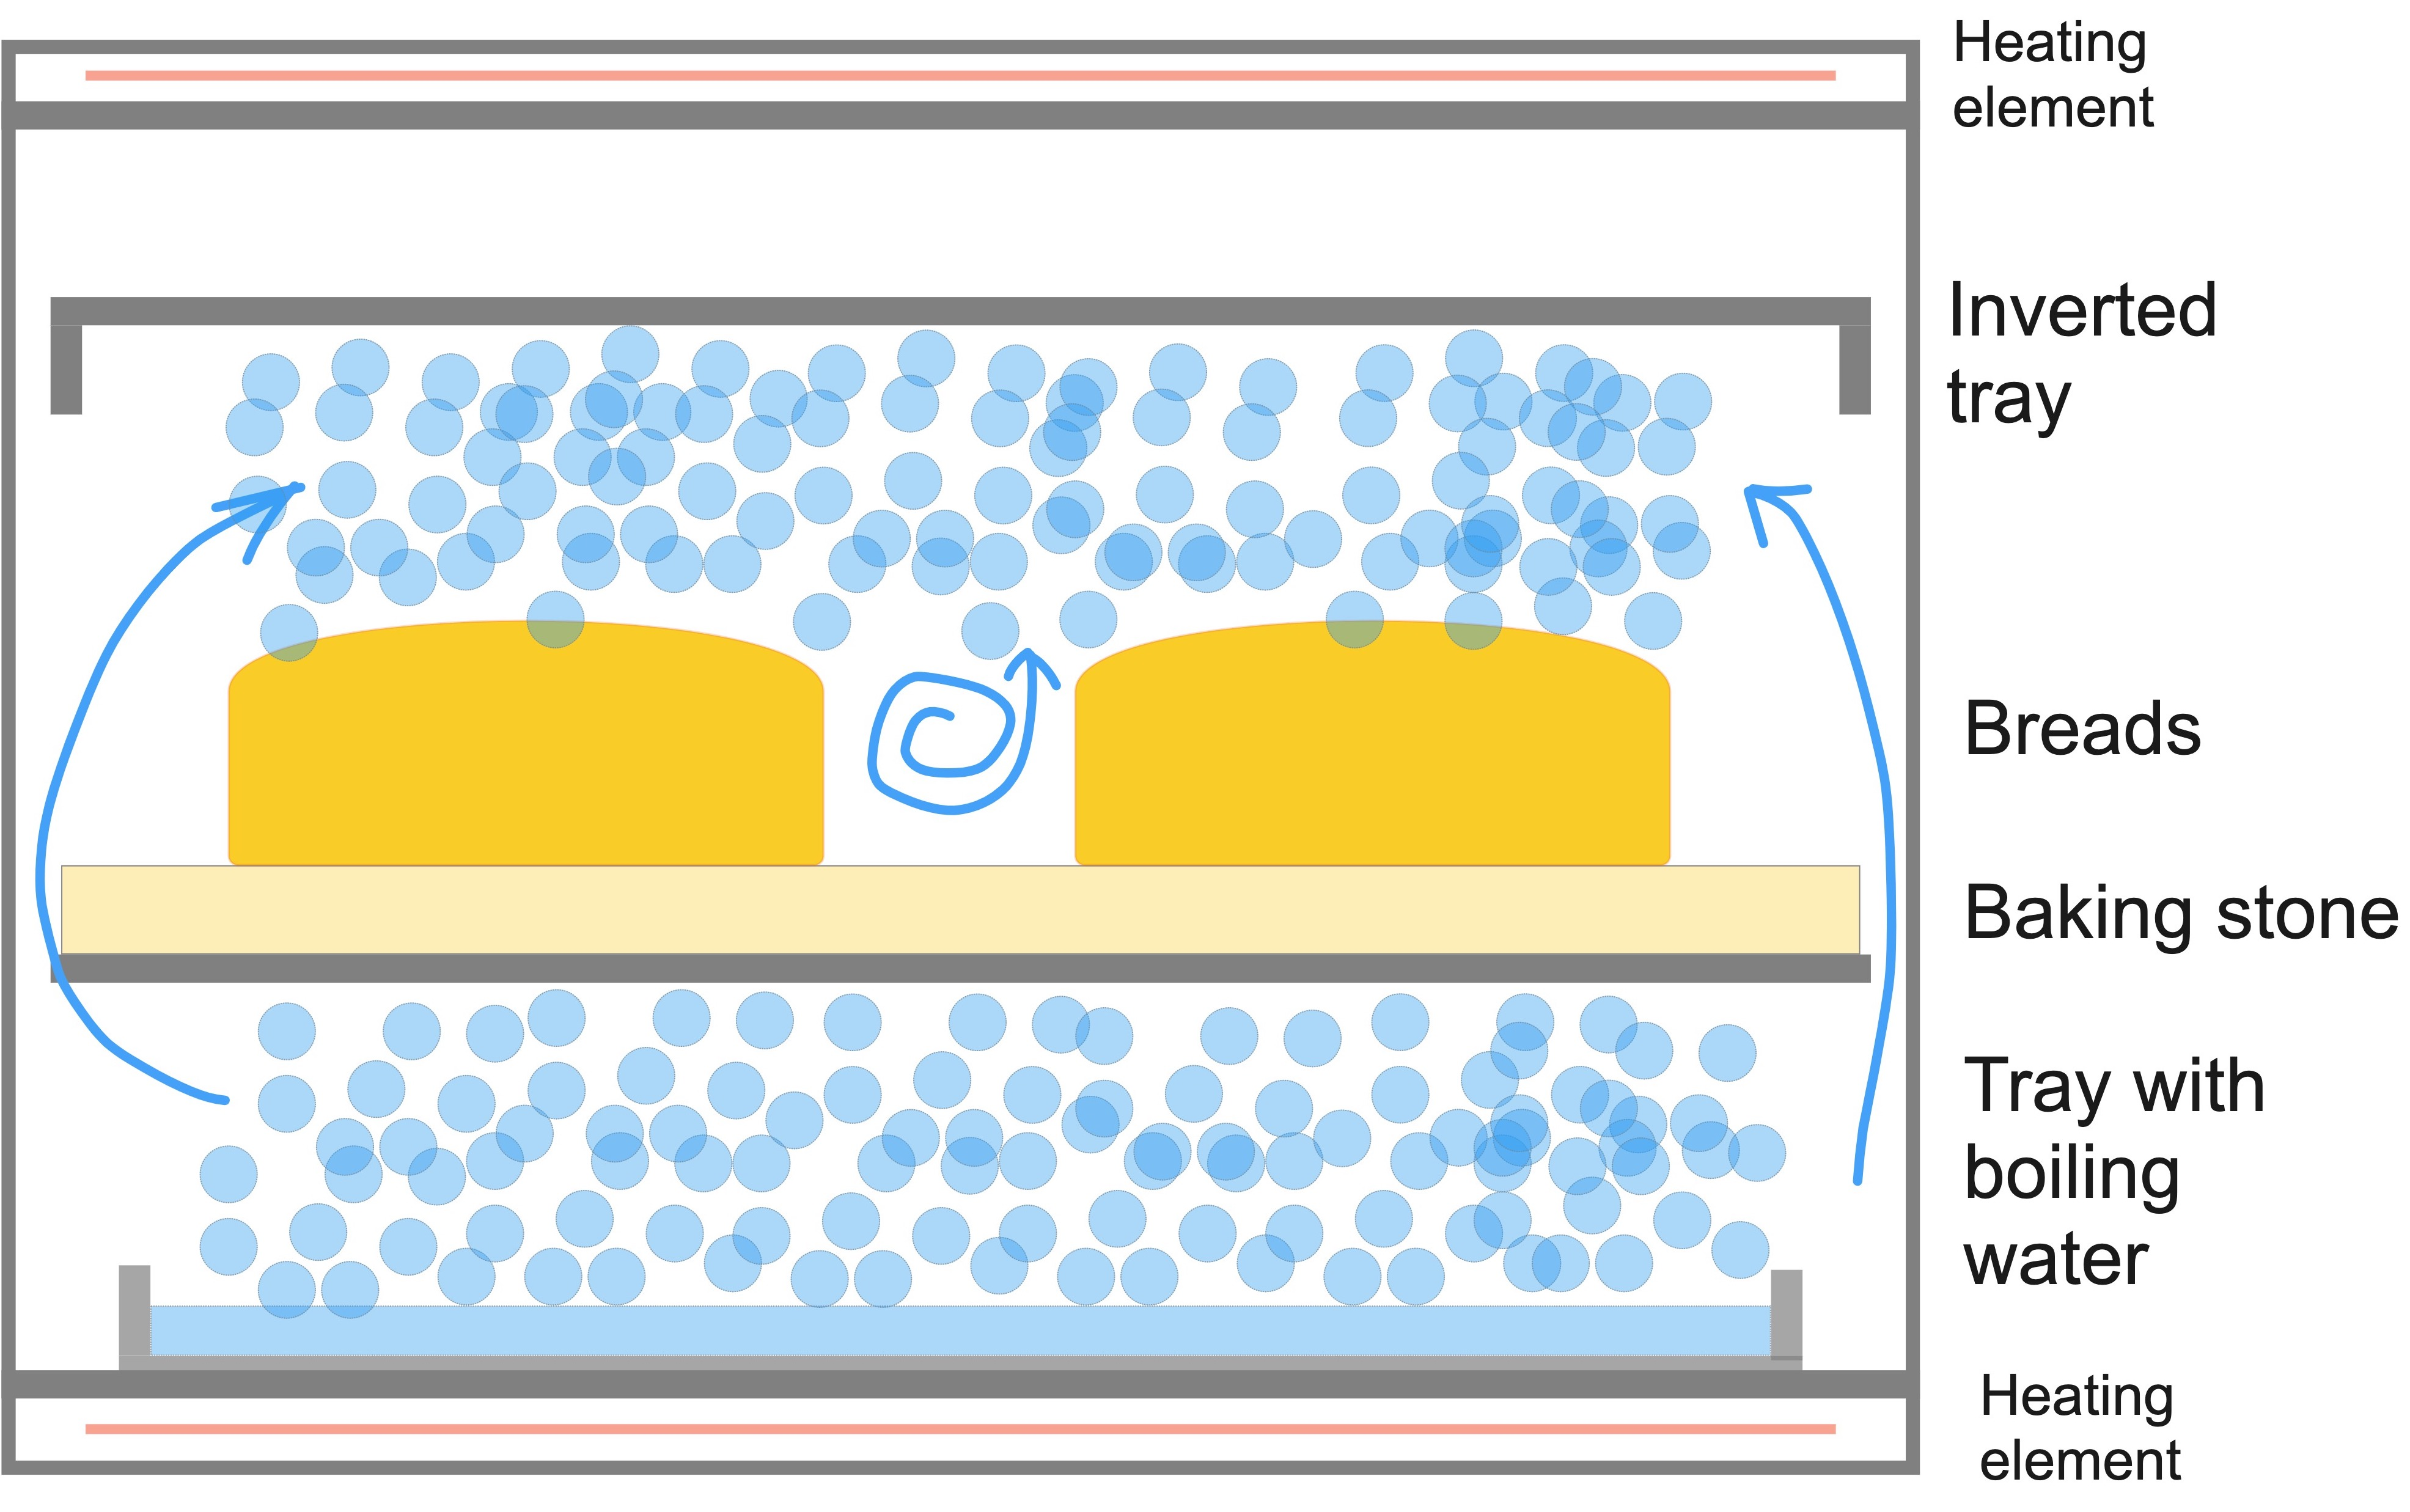
\includegraphics[width=\textwidth]{baking-process-steam.jpg}
  \caption[Steam building with inverted tray]{How steam builds in your oven
      using the later described inverted tray method.}
\end{figure}

Normally, under high heat a crust would form. Just like
if you were to bake vegetables in your home oven, at some point
they become darker and crisper. This is the same thing that
happens with your dough. You want to delay this process
as long as possible until your dough no longer expands.
Expansion stops when most of the microbes have died and
the evaporating water no longer stays inside the alveoli.
The stronger the gluten network, the more gas can be retained
during the baking process. This gluten network at some point
loses its ability to contain gas as the temperature heats
up. The dough stops increasing in size. The steam plays
an important role as it condenses and evaporates on top
of your dough. The surface temperature is rapidly increasing
to around  \qty{75}{\degreeCelsius} (\qty{160}{\degF}). At this temperature the gel starts
to build. This gel is still extensible and allows expansion.
Without the steam, the dough would never enter the gel stage,
but instead directly go to the Maillard reaction zone. You
want your dough to stay in this gel stage as long as possible
to achieve maximum expansion\footnote{You can remove your
dough from the oven after 5~minutes to see the gel. You will notice
that it holds the dough's structure. It has a very interesting consistency.}.

\begin{figure}[!htb]
  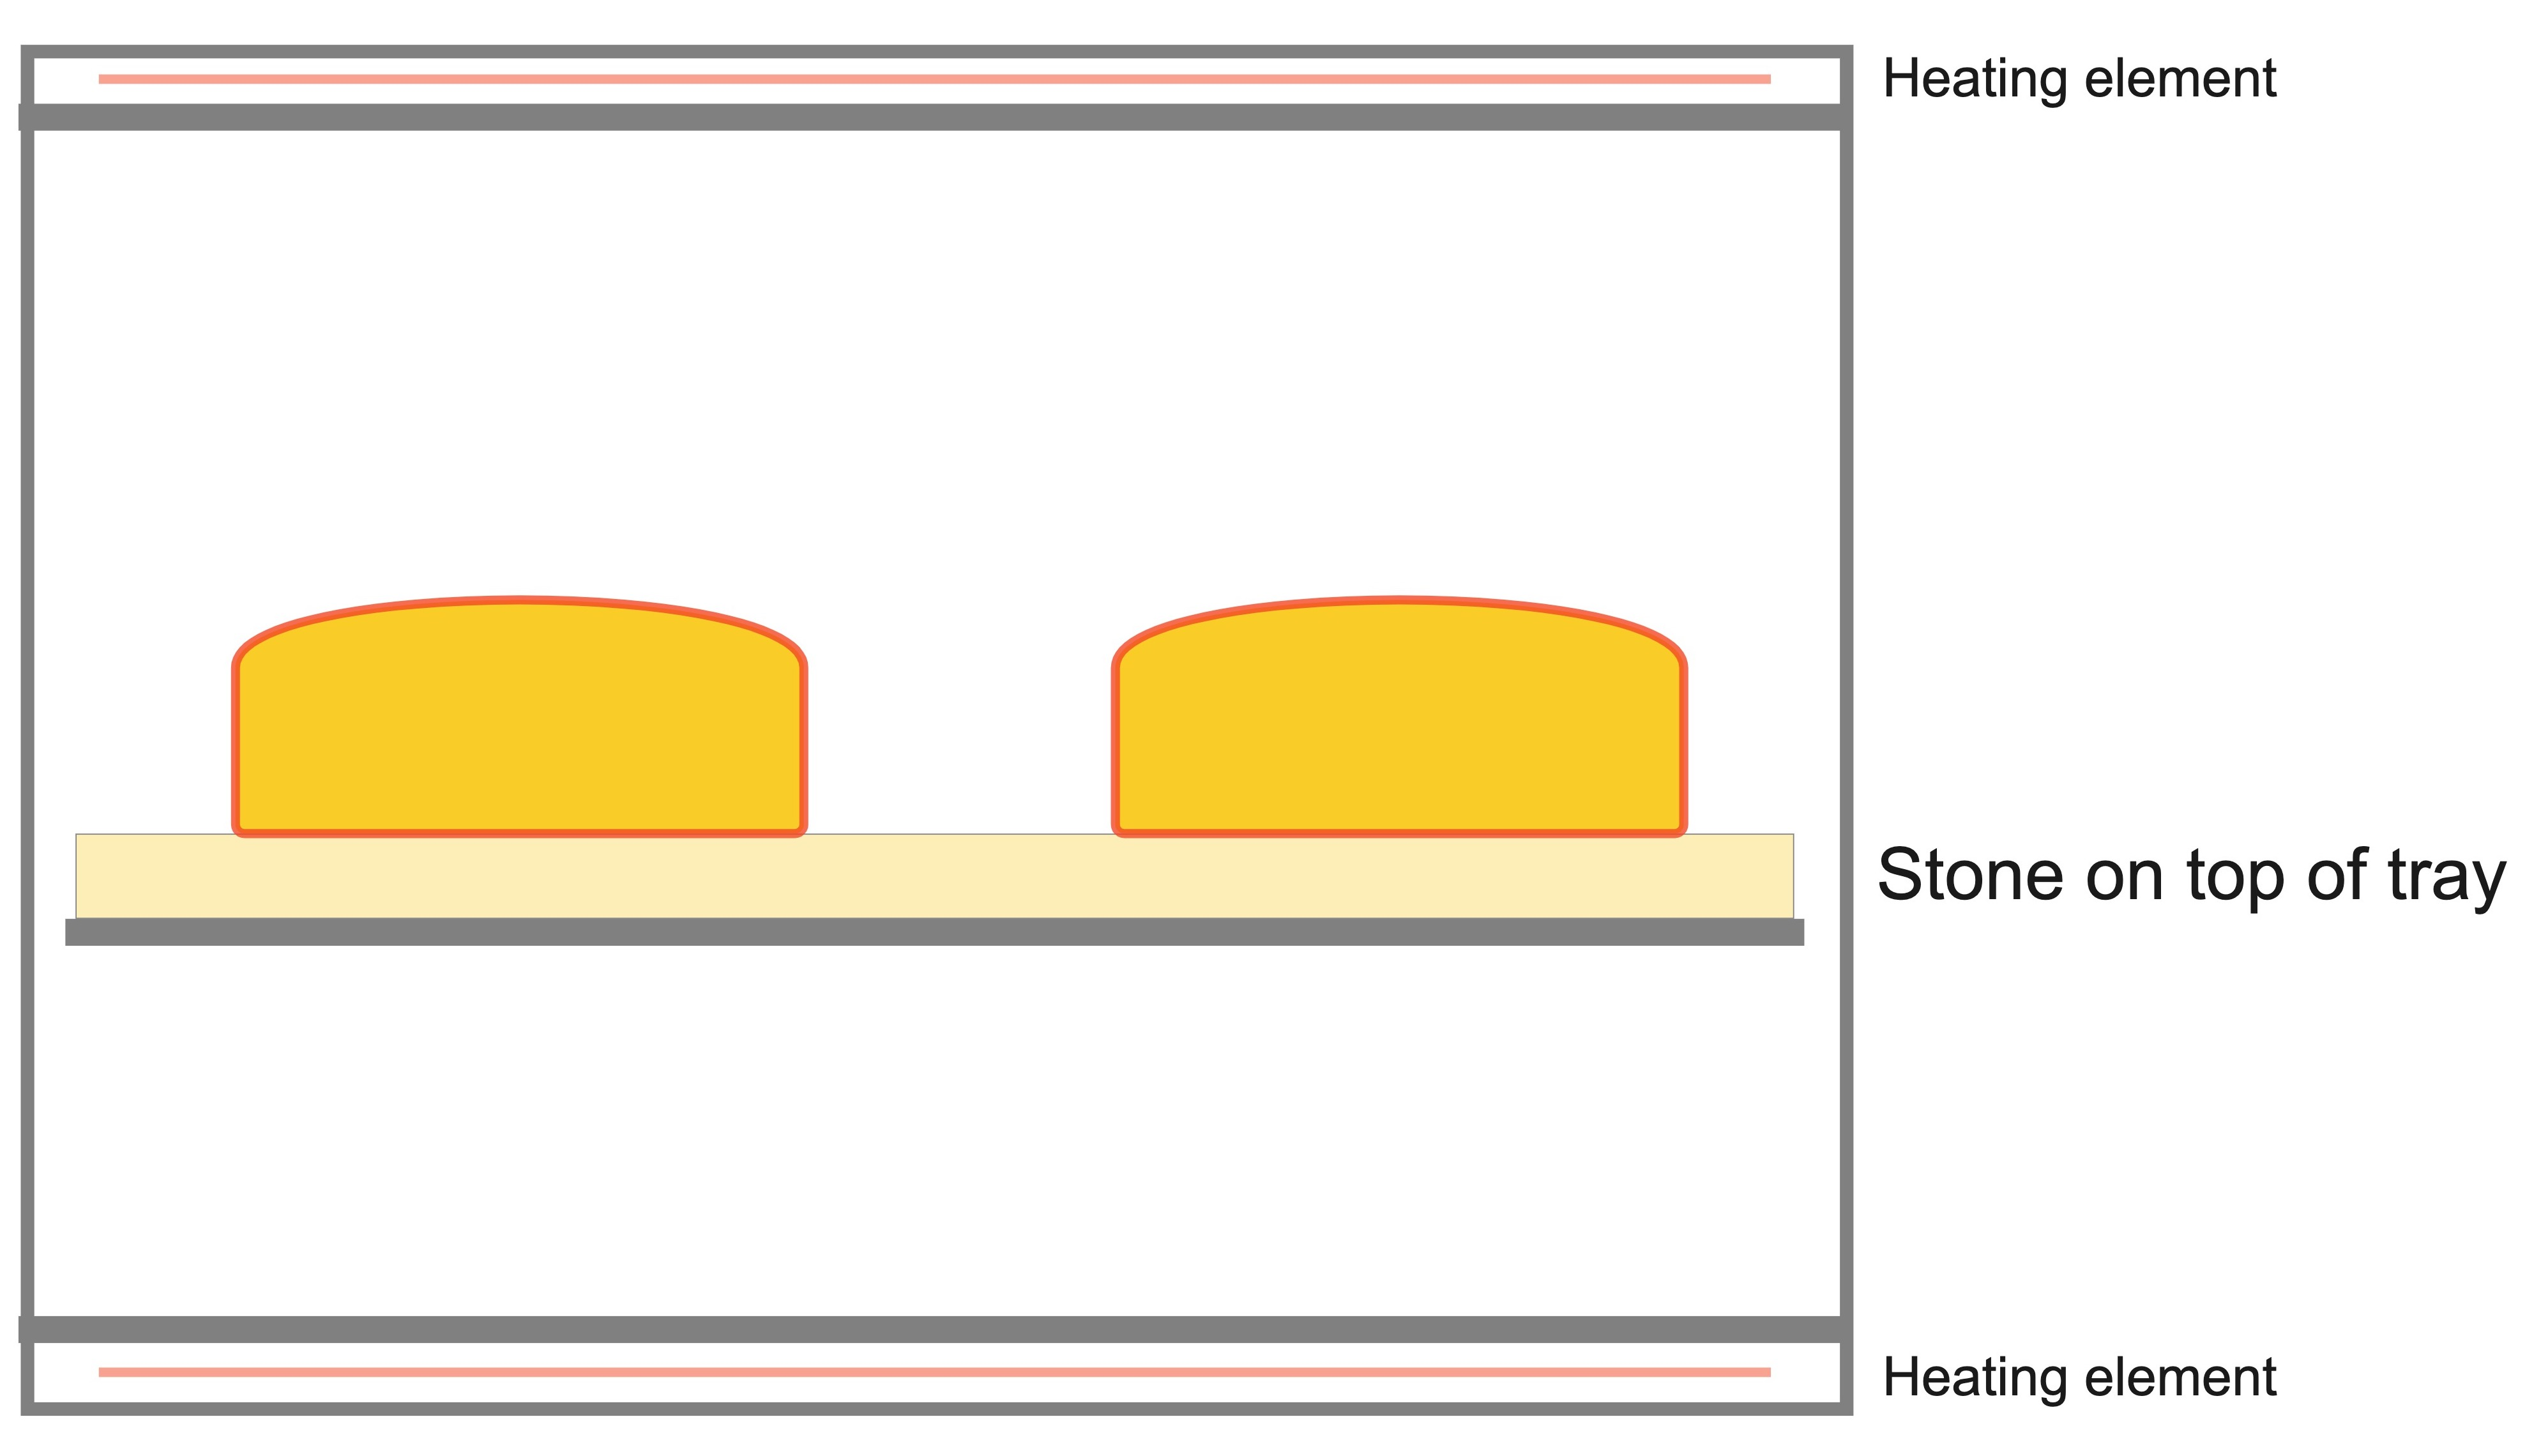
\includegraphics[width=\textwidth]{baking-process-stage-2.jpg}
  \caption[Baking step~2, without steam]{The second stage of the bake is done
      without steam to build a thicker, darker crust.}
\end{figure}

When not steaming enough, you will notice that the scoring
incisions do not properly open up during the bake. They stay
closed as the dough is unable to push through the crust.

Another common sign is that you have larger pockets
of air towards the crust of your dough. As the dough increases
vertically, expansion is halted by the crust. The pockets
of air converge into larger pockets as the pressure increases.
This can also happen when you are baking at too high a temperature.

The more you steam, the softer your dough's crust is. You will never
enter the Maillard and caramelization stage. This
is the reason why the source of steam is removed
for the second stage of the bake. No more expansion can
happen and you can focus on building a crust. If you
would like a soft crust, you can steam your dough all the
way.

\begin{figure}[!htb]
  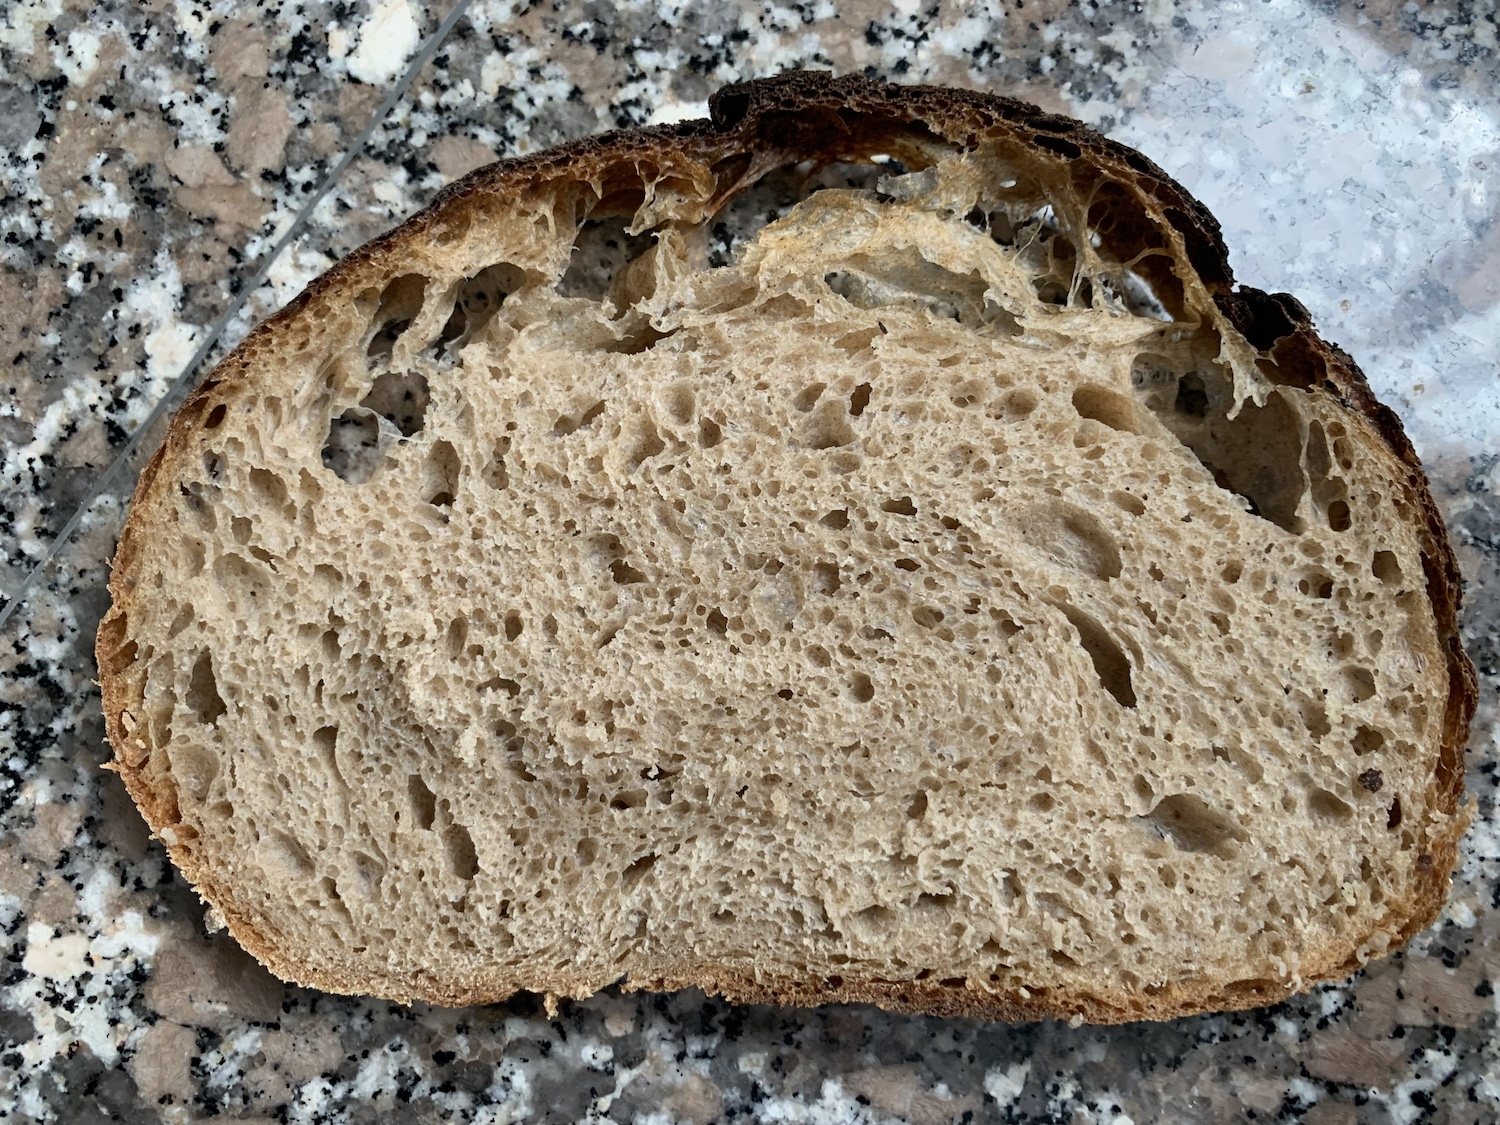
\includegraphics[width=\textwidth]{baking-too-hot}
  \caption[Bread baked too hot]{A submission by Karomizu showing a bread that
      has been baked at too high a temperature or with too little steam. Note
      the large pockets of air towards the crust. They are a typical
      indicator.}
\end{figure}

\section{Dutch ovens}

\begin{figure}[!htb]
  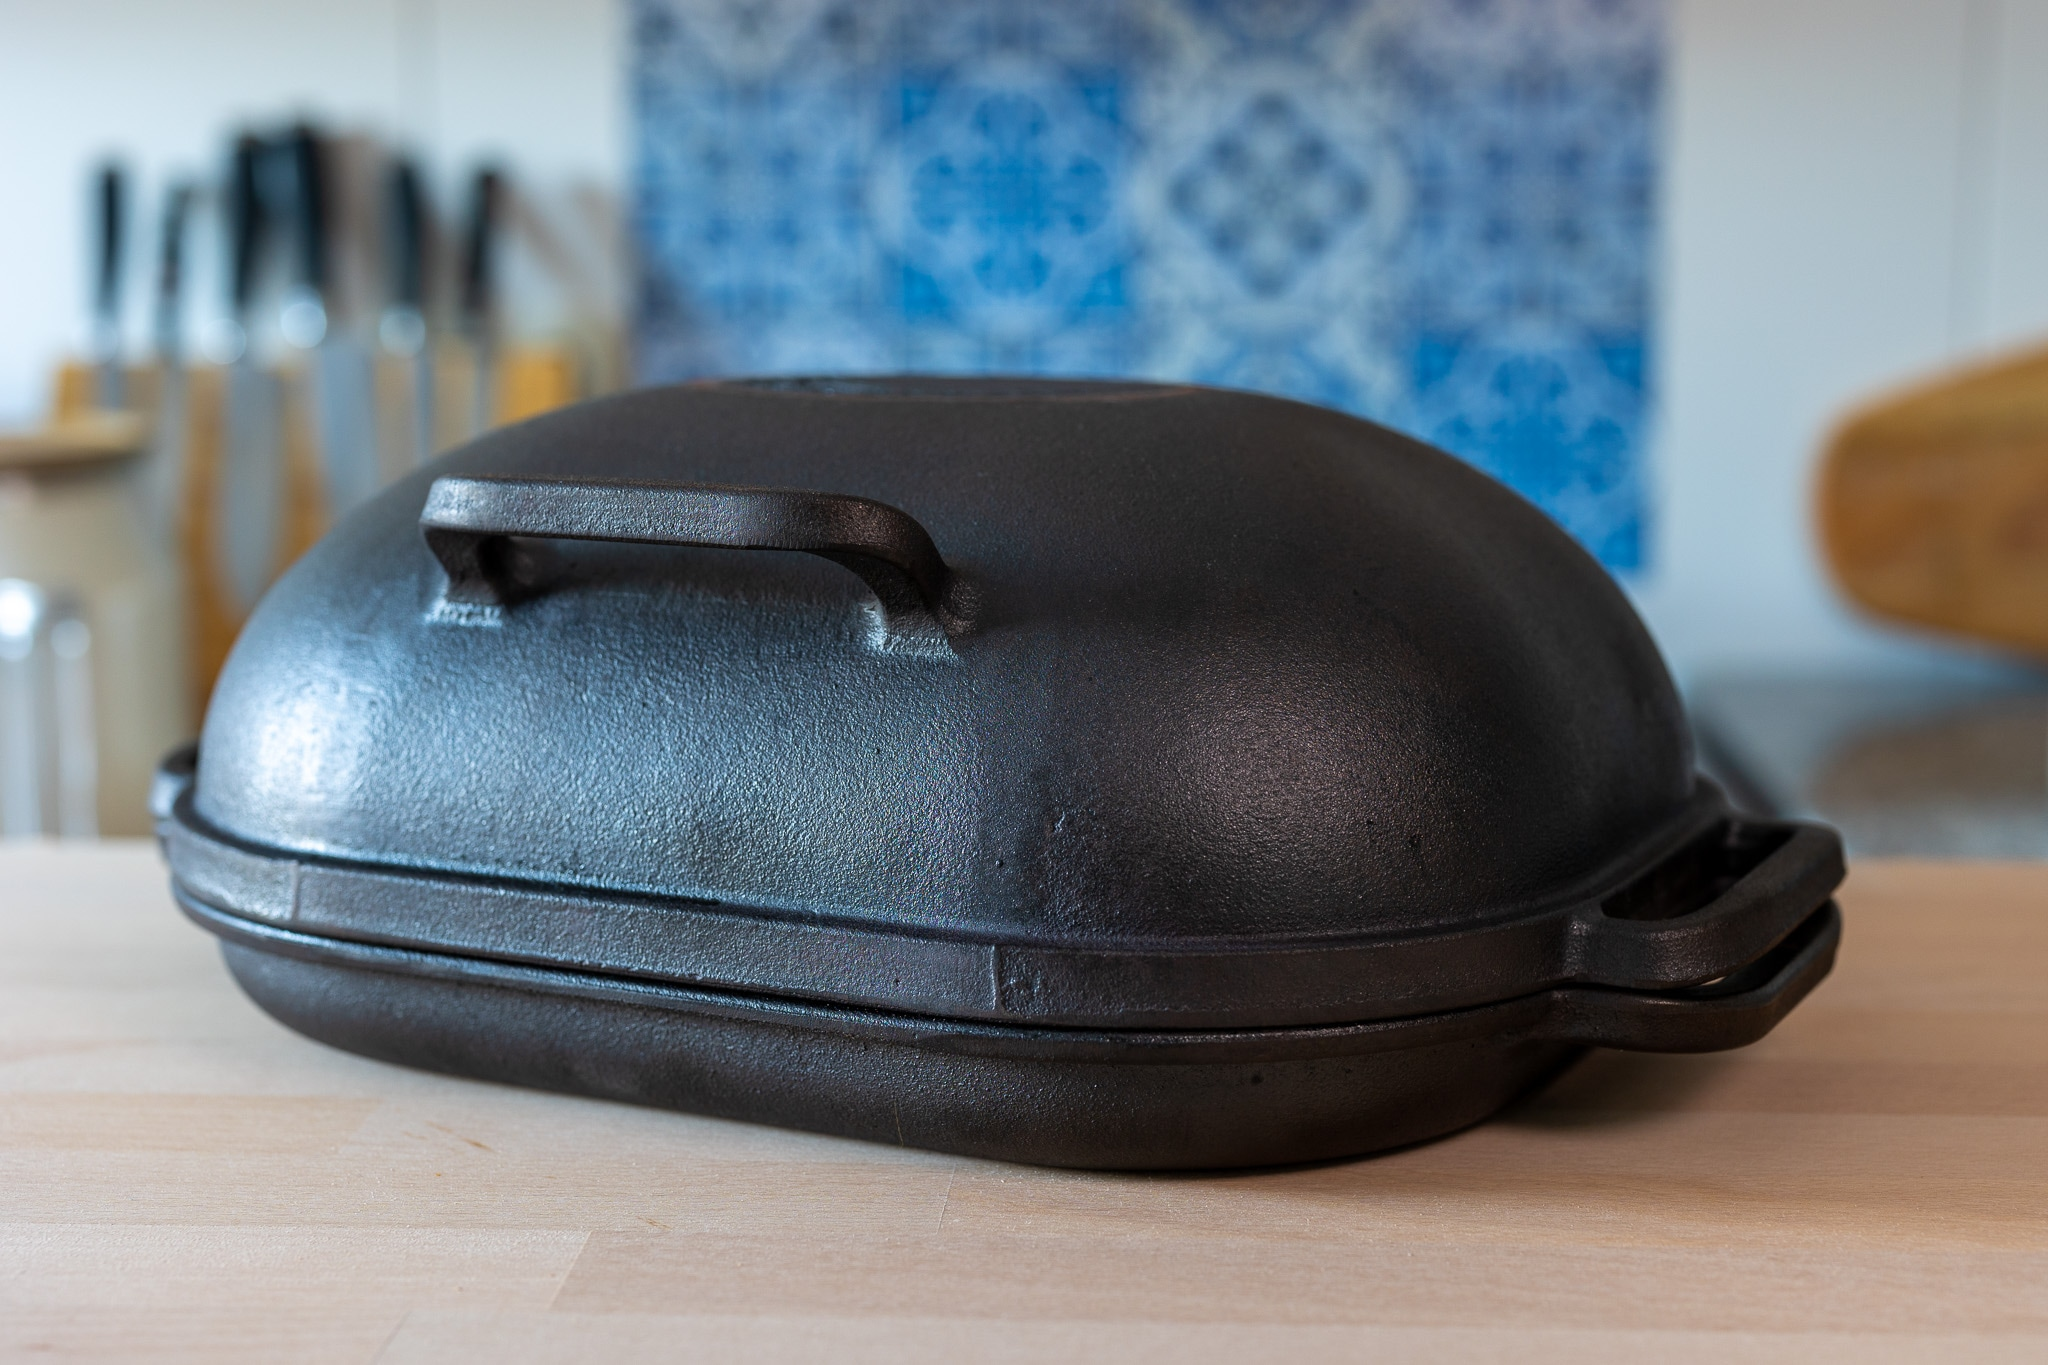
\includegraphics[width=\textwidth]{dutch-oven-example}
  \caption[Picture of dutch oven]{An example of a dutch oven. Some are also
      made out of enameled cast iron, others are made out of clay and some
      feature a glass lid.  They all work similarly by entrapping some of the
      steam created during the baking process. The steamy environment allows
      the bread to rise further and thus have more oven spring and feature a
      fluffier crumb.}%
\end{figure}

\begin{flowchart}[!htb]
\begin{center}
  \begin{tikzpicture}[node distance = 3cm, auto]
  \node [start] (heat_oven) {Preheat DO to \qty{230}{\degreeCelsius} (\qty{446}{\degF}) for 30~minutes};
  \node [block, right of=heat_oven] (remove_oven) {Remove DO from oven };
  \node [block, right of=remove_oven] (open_load_dough) {Open DO \& load your dough};
  \node [block, right of=open_load_dough] (score) {Score your dough};
  \node [block, right of=score] (spritz) {Spritz dough with water};
  \node [block, below of=spritz] (close) {Close DO};
  \node [block, left of=close] (back_oven) {Place DO back in oven};
  \node [block, left of=back_oven] (bake) {Bake 30~minutes at \qty{230}{\degreeCelsius} (\qty{446}{\degF})};
  \node [decision, below right= 5cm and -1 cm of heat_oven]  (is_ready_check)
        {Core temperature \qty{92}{\degreeCelsius} (\qty{197}{\degF})?};
  \node [block, below of=is_ready_check, node distance=4cm] (wait_5_minutes) {Wait\\ 5 minutes};
  \node [block, right of=is_ready_check, node distance=4cm] (remove_do_lid) {Remove DO lid};
  \node [decision, right of=remove_do_lid, node distance=3.5cm] (dark_enough_decision) {Crust color dark enough?};
  \node [success, below of=dark_enough_decision, node distance=4cm] (finish_baking) {Bread is finished};
  \node [block, right of=dark_enough_decision, node distance=3.5cm] (bake_5_more_minutes) {Bake another 5~minutes};
  \path [line] (heat_oven) -- (remove_oven);
  \path [line] (remove_oven) -- (open_load_dough);
  \path [line] (open_load_dough) -- (score);
  \path [line] (score) -- (spritz);
  \path [line] (spritz) -- (close);
  \path [line] (close) -- (back_oven);
  \path [line] (back_oven) -- (bake);
  \path [line] (bake.west) -- node{} ++(-2, 0) -| (is_ready_check.north);
  \path [line] (is_ready_check) -- node{yes} (remove_do_lid);
  \path [line] (is_ready_check) -- node{no} (wait_5_minutes);
  \path [line] (wait_5_minutes.west) -- node{} ++(-1.5, 0) |- (is_ready_check.west);
  \path [line] (remove_do_lid) -- (dark_enough_decision);
  \path [line] (dark_enough_decision) -- node{yes} (finish_baking);
  \path [line] (dark_enough_decision) -- node{no} (bake_5_more_minutes);
  \path [line] (bake_5_more_minutes.east) -- node{} ++(1, 0) -- node{} ++(0, 2.3) -| (dark_enough_decision.north);
\end{tikzpicture}

  \caption[Baking process with a dutch oven]{A visualization of the baking
      process using a dutch oven (DO). The dough is steamed for the first half
      of the bake and then baked without cover for the second half of the
      bake. The desired darkness and thickness of the crust depends on your
      personal preference. Some bakers prefer a lighter crust and others a
      darker.}%
  \label{fig:dutch-oven-process}
\end{center}
\end{flowchart}

Dutch ovens are an ideal way to bake with a lot of
steam. They are not fully sealed. Regardless though,
as water evaporates from your dough, it will create a steamy
environment allowing your dough to rise. It
makes baking in a home oven very easy.

When using a Dutch oven, make sure to preheat it properly,
this way your dough will not stick to it. You can also
use additional semolina flour or parchment paper. Another
good trick is to spritz your dough with a bit of water.
To create more steam, you could also place a small ice cube
next to your main dough.

I~have been using a Dutch oven myself for a long time. They
have issues though. They are relatively heavy. It is dangerous
to operate hot cast iron ovens. Especially when working with steam,
you have to be very careful. Furthermore,
they are expensive to buy. If your Dutch oven is made out
of cast iron you have to season it from time to time. This takes
time.

The biggest disadvantage, though, is
capacity. You can only bake a single piece of bread at a time,
as the size of the Dutch oven is limited.
In many cases, it makes sense to bake multiple
loaves in one go. It makes the whole process more
efficient as you have to knead less per loaf. The time it
takes to make one loaf is significantly reduced. Furthermore,
you don't require as much energy. You don't have
to preheat your oven twice for each loaf.

An additional disadvantage of Dutch ovens is the
need to move very hot and heavy cast iron\footnote{%
  Some of them can weigh up to 10 kg. Moving them is quite
  a tedious exercise. Especially if the cast iron is
  heated you have to be very concise with your movements.
  Despite doing my best I have a few scars on my
  hands and arms from operating the Dutch ovens.
}.
You will need to be very careful and ideally use
heat-resilient gloves when touching your Dutch oven.

Furthermore, some of the Dutch ovens come at a hefty
price tag. Especially for new bakers buying a Dutch oven on
top of other tools can be quite a hefty investment. For
this reason, I advocate the inverted tray method visualized
in the next section. In case you do not own an oven consider trying
the simple flatbread recipe which is baked in a pan. Please
refer to Section~\ref{section:flat-bread-recipe} for more details.


\section{Inverted tray method}

The inverted tray method simulates a Dutch oven.
By placing another tray on top of your dough, the steam
created from the dough and water source stays
around your dough.

\begin{figure}[!htb]
\begin{center}
  \begin{tikzpicture}[node distance = 3cm, auto]
  \node [block] (init) {\footnotesize Place water tray and stone in oven};
  \node [block, right of=init] (heat_oven) {\footnotesize Heat oven to  \qty{230}{\degreeCelsius} (\qty{446}{\degF}) for 30~minutes};
  \node [block, right of=heat_oven] (score_your_dough) {\footnotesize Score your dough};
  \node [block, right of=score_your_dough] (spritz) {\footnotesize Spritz your dough with water};
  \node [block, right of=spritz] (load_tray) {\footnotesize Place non-preheated inverted tray in oven};
  \node [block, below of=load_tray, node distance=4cm] (load_doughs) {\footnotesize Load doughs into oven};
  \node [block, left of=load_doughs, node distance=3cm] (load_water) {\footnotesize Place water in heated water tray};
  \node [block, left of=load_water, node distance=3cm] (bake) {\footnotesize Bake 30~minutes or until core temperature is  \qty{92}{\degreeCelsius} (\qty{197}{\degF})};
  \node [block, left of=bake, node distance=3cm] (remove_steam) {\footnotesize Remove steam source and top tray};
  \node [block, left of=remove_steam, node distance=3cm] (finish) {\footnotesize Bake at least another 10~minutes or until crust has your desired color};
  \path [line] (init) -- (heat_oven);
  \path [line] (heat_oven) -- (score_your_dough);
  \path [line] (score_your_dough) -- (spritz);
  \path [line] (spritz) -- (load_tray);
  \path [line] (load_tray) -- (load_doughs);
  \path [line] (load_doughs) -- (load_water);
  \path [line] (load_water) -- (bake);
  \path [line] (bake) -- (remove_steam);
  \path [line] (remove_steam) -- (finish);
\end{tikzpicture}

  \caption[Inverted tray baking process]{A schematic visualization the
  inverted tray baking method that works great for home ovens.}%
  \label{fig:inverted-tray-process}
\end{center}
\end{figure}


The biggest advantage of this method compared to the
Dutch oven is scalability. You can bake multiple loaves
at the same time. In my case that is around 2 freestanding
loaves and 4 loaves in a loaf pan.

For the inverted tray you will need the following tools:
\begin{itemize}
\item 2 trays
\item 1 heat resistant bowl
\item Boiling water
\item Oven gloves
\item (Optional) Parchment paper
\end{itemize}

\begin{figure}[!htb]
  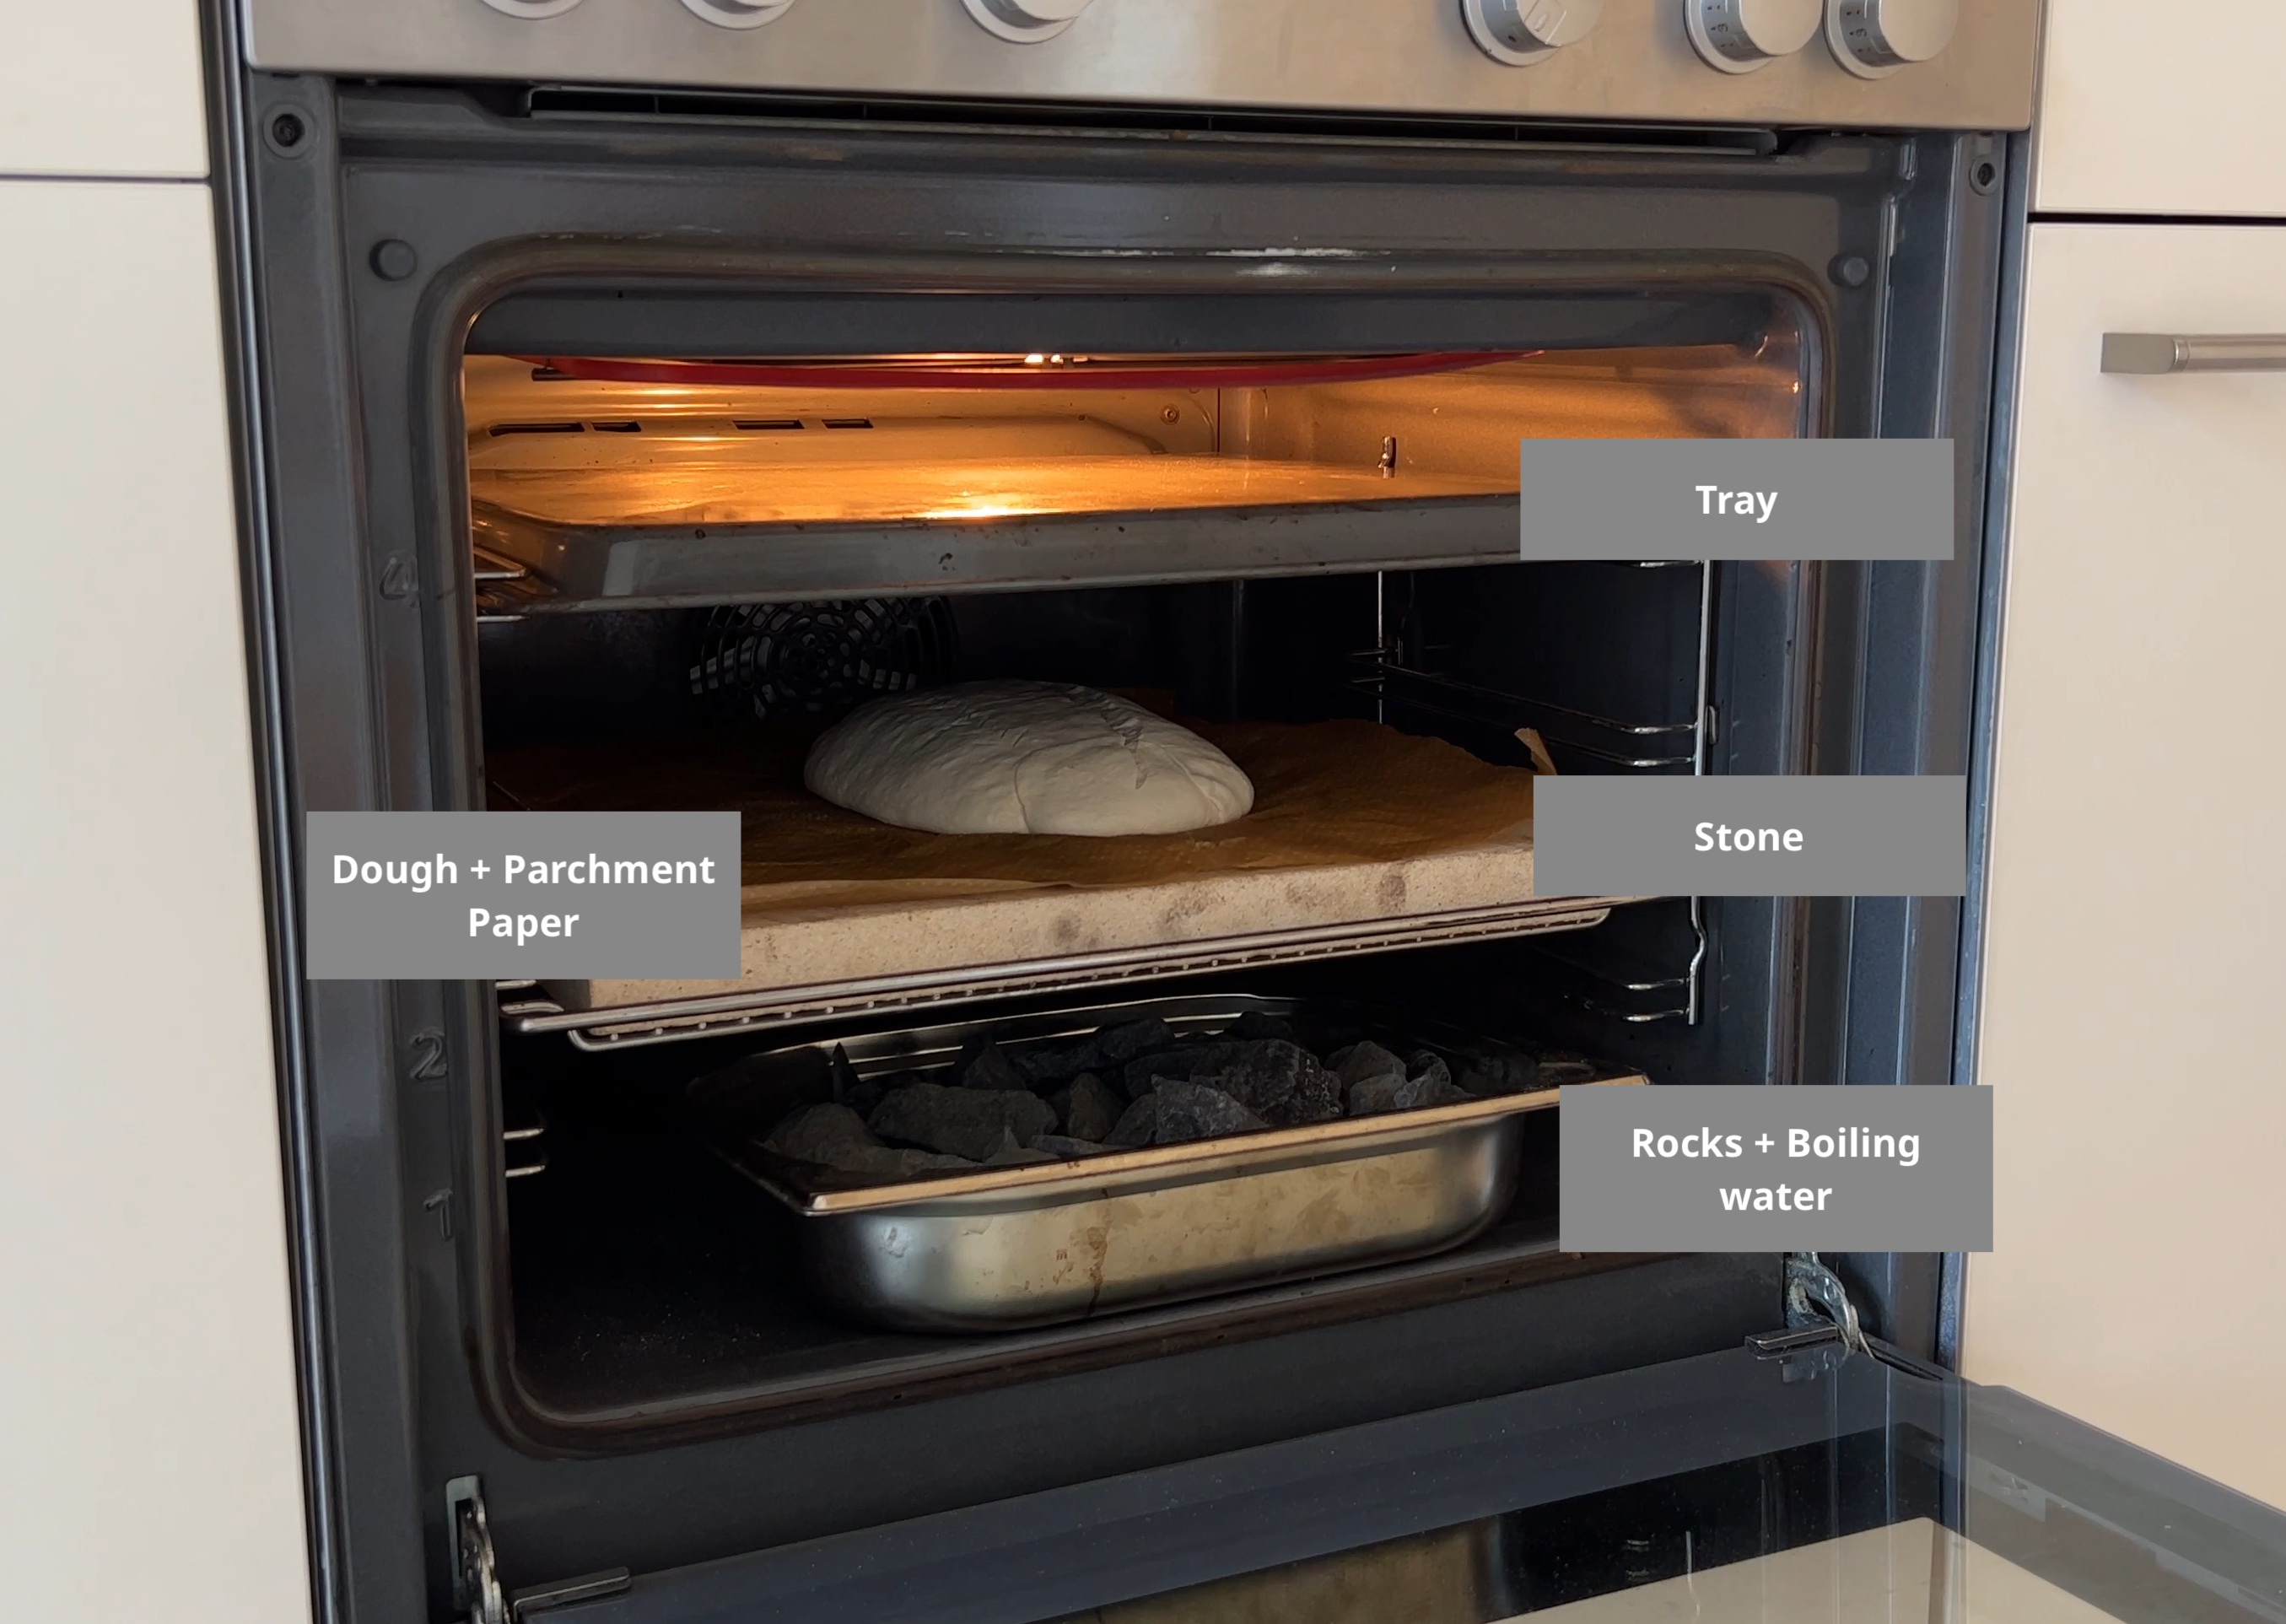
\includegraphics[width=\textwidth]{baking-example.jpg}
  \caption{My home oven setup.}
\end{figure}

These are the steps to follow with the inverted tray method:
\begin{enumerate}
\item Preheat the oven to around  \qty{230}{\degreeCelsius} (\qty{446}{\degF}) and
preheat one of the trays.
\item Bring water to boil.
\item Place your loaves on a piece of parchment paper. You
can also place each on a tiny piece of parchment paper.
This makes loading the dough easier. If you don't
have it or don't want to use it, you can opt for
semolina flour. It helps to make the tray nonstick.
\item Take out your hot tray and place it
on a cooling rack or on something else that
is heat resistant.
\item Score your doughs.
\item Place your doughs on the hot tray.
\item Place the cold tray in your oven in an inverted position.
\item Move your hot tray including the loaves back
to the oven.
\item Place the boiling water in the heat-resistant
water bowl. I~have added rocks to it, as it helps
to improve the steam even further. This is optional.
\item Close the oven.
\item After 30~minutes remove the top tray. Also remove the bowl with water.
\item Finish baking your bread until you have reached your desired
crust color. In my case this is another 15--25~minutes typically.
\end{enumerate}

\section{Conclusions}

\begin{table}[!htb]
    \begin{center}
        % TODO: Not great Looking... 
\begin{tabular}{@{}p{0.25\textwidth}ccc@{}}
\toprule
\thead{Oven type}  & \thead{Plain (no tools)} & \thead{Inverted tray} & \thead{Dutch oven} \\ \midrule
Gas                & No                       & No                    & Yes                 \\ \midrule
Convection (Fan always on) & No               & No                    & Yes                 \\ \midrule
Convection (Fan can be disabled) & No         & Yes                   & Yes                 \\ \midrule
Steam              & Yes                      & Yes                   & Yes                 \\
\bottomrule
\end{tabular}

        \caption[Different oven types]{An overview of different oven types and their
            different baking methods.}
    \end{center}
\end{table}

Depending on your home oven, a different method
of steaming may be used. Generally most ovens
are made to vent out most of the steam during the
bake. They are typically not fully closed. During
baking you want to dry out whatever you are baking.
This is ideal if you are roasting vegetables and
want them to dry out. For baking though, this is
highly problematic. As described earlier, you
want there to be as much steam as possible.

If you are using a gas-based oven, the only option
is to utilize a Dutch oven. The same is true when you
are using a convection oven with a fan that
cannot be disabled. When using a convection
oven with a fan that can be turned off, you can
opt to use the cost-efficient inverted tray
method.

If you are in the luxurious
position of owning a steam oven, things are easier.
Just activate the steam function and you are
good to go. Placing an additional tray on top of your
dough during the bake helps to bake with indirect
heat. You remain in the gel zone longer and
will experience more oven spring.
